The QCD axion arises as a by-product of the most successful solution to the Strong CP Problem in the Standard Model \citep{PecceiQuinn:1977}. 
The abundance of axions is set by the Peccei-Quinn symmetry breaking scale $f_a$ with a value
\begin{equation}
\Omega_a\sim\left(\frac{f_a}{10^{11-12}\,{\rm GeV}}\right)^{7/6}.
\end{equation}
This expression may be altered due to the temperature-dependence of the axion mass and ignorance about whether the Peccei-Quinn symmetry breaks before or after inflation. 
Axion theory gives no {\it a priori} prediction for the axion mass; however, in the context of dark matter composed of QCD axions, an axion mass $m_\phi< 10^{-3}$ eV ($10^{-39}$ kg). 
If the initial mass alignment angle is order unity, this yields a QCD axion mass of $\roughly 10^{-5}$ eV ($10^{-41}$ kg) is usually considered.  
\ADW{Please check Chanda!}

A broader category of axion-like particles (ALPs) possess QCD axion-like potentials, but do not obey the same coupling between particle mass and symmetry breaking scale. ALPs are a broad class of light scalar particles which obey a shift symmetry $\phi \rightarrow \phi + 2\pi n$. They can be motivated by string theory, where there are many moduli with axion-like potentials. ALPs can be sufficiently different from the QCD axion so as to produce notably different astrophysical phenomenology. 

Astrophysical constraints on ALPs generally come from a hypothetical coupling of the ALP with photons and/or electrons. 
\begin{equation}
    \mathcal{L} = -\frac{1}{2} \partial_\mu\phi\partial^\mu\phi + \frac{1}{2}m_\phi^2 \phi^2 - \frac{1}{4}g_{\phi\gamma}F_{\mu\nu}\tilde{F}^{\mu\nu}\phi,
\end{equation}
where $g_\phi\gamma$ is the photon-axion coupling and $F^{\mu\nu}$ is the electromagnetic field tensor (and $\tilde{F}$ its dual). There are additional couplings for example to nucleons, but they are not expected to be relevant to LSST science.  

Astrophysical observations place the only known lower bound on the mass of ALPs and other non-thermally produced particles, commonly described as ``fuzzy'' dark matter. The Compton wavelength of these particles is constrained to be smaller than the size of the smallest galaxy, setting a lower limit on particle mass at $m \gtrsim 10^{-22}$ eV. The scalar nature of the axion along with its high abundance in the early universe can -- what was the rest of this sentence? The mass of the particle also determines the significance of quantum pressure in structure formation.



%ADW: I think the paragraphs below have slightly too much much detail, for this report. It would be good to talk about axion stars, galaxy caustics, and anomalous energy loss in stellar populations and SN.

%CPW, 10/29/2018: I think some of it should be reintroduced, but I have shortened and edited to suggest these are different scenarios under consideration.
%\subsubsection{Axions and Structure Formation}
There has been significant debate in the literature about the astrophysical phenomenology of the QCD axion. Sikivie and Yang (2009) noted that because the axion is a scalar with high abundance in the early universe (circa matter-radiation equality), the axion could potentially settle into a Bose-Einstein condensate state. By ``Bose-Einstein condensate'' one has loosely meant that all particles can be described using one coherent ground state wave function. What is distinct about Sikivie and Yang's proposal is not so much the idea that the axion might begin as a BEC -- this seems likely (although making this statement formal is an open problem) -- but rather once the particles experience perturbations, do they remain in a BEC state? SY argue that during the radiation-dominated era, axions will rethermalize into BECs with a Hubble-scale correlation length, with significant phenomenological implications such as low-redshift galaxy scale (tens of kpc) caustics with a non-spherical topology. These are distinct from the spherical topology predicted by Bertschinger for WIMPs. 

\citet{1412.5930} showed that rather than a Hubble-scale correlation length at matter-radiation equality that leads to galaxy halo phenomenology, a particle such as the QCD axion, which has an attractive self-interaction, in an attractive gravitational potential will not stably have large scale correlations. Rather, axions in this early universe era will form coherent clumps that have been called Axion stars or Bose stars (see Kolb and Tkachev 2000) but should more reasonably probably be called axteroids (originating with Anna Watts). This proposal has a distinct phenomenology and LSST observations of rotation curves, providing insights into caustics around nearby galaxies, may help distinguish between the two.

Complicating LSST's capacity to distinguish between models is the possibility of degeneracy between the SY model and other axion-like particle phenomenologies. Both of the aforementioned scenarios, which have kicked off significant debate and renewed interest in Bose-Einstein condensed axion phenomenology, focus on the QCD axion in a mass range of around $10^{-5}$ eV. There is an extensive literature regarding axion phenomenology beyond the QCD axion and this mass range, e.g. ultralight axions (ULA) and fuzzy dark matter (FDM). In ULA/FDM scenarios, the De Broglie wavelength of the particle is such that the coherent wave can be halo-scale, which may give distinct stellar density distributions, which LSST will measure, than the SY proposal or the clump scenario.
\TT{We should also mention the dark photon}
\ADW{Would we want to include some discussion of soliton cores from fuzzy DM?}

LSST will be able to probe axion dark matter in the following ways:
\begin{itemize}
    \item Caustics around Nearby Galaxies \CPW{11.25 Dealt with, now?}
    \item Anomalous Cooling in Stellar Populations 
    \begin{itemize}
        \item White dwarf luminosity function
        \item Globular cluster
        \item Cepheids / blue loop?
    \end{itemize}
    \item Supernova Observations
    
\end{itemize}

\begin{figure}
\centering
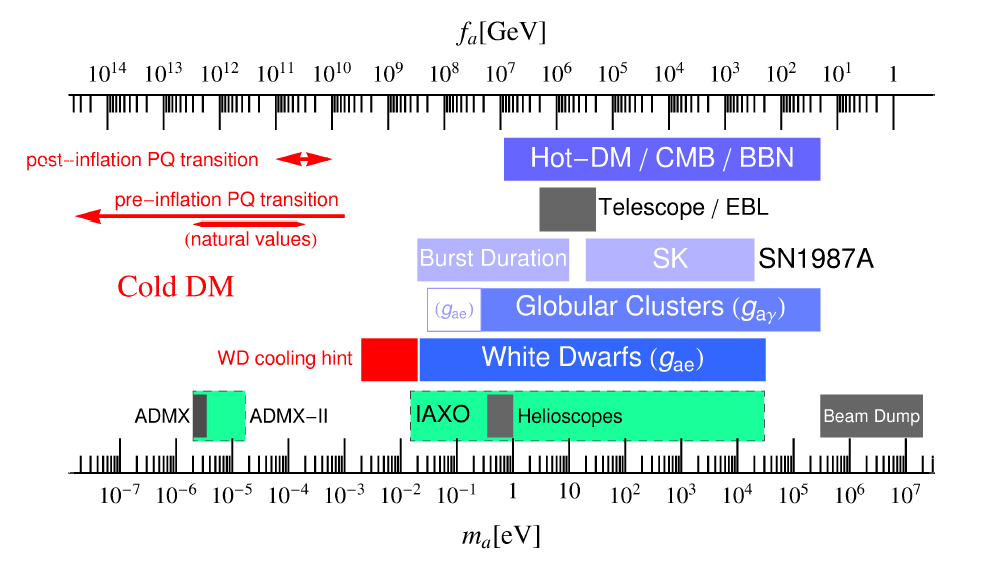
\includegraphics[width=0.6\columnwidth]{axions.png}
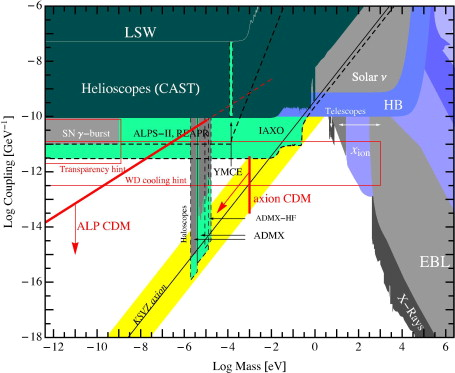
\includegraphics[width=0.39\columnwidth]{alps.jpg}
\caption{Maybe something like on the left for axion constraints 
Taken from \citep{Redino:2015} \url{https://arxiv.org/abs/1512.06822}. Right: Figure that could be used for ALP constraints \citep{Ringwald:2012} \url{https://arxiv.org/abs/1210.5081}}
\end{figure}

%ORIGINAL CUT FROM MAIN DOC
%ADW: I think the paragraphs below have slightly too much much detail, for this report. It would be good to talk about axion stars, galaxy caustics, and anomalous energy loss in stellar populations and SN.

%There has been significant debate in the literature about the astrophysical phenomenology of the QCD axion. Sikivie and Yang (2009) noted that because the axion is a scalar with high abundance in the early universe (circa matter-radiation equality), the axion could potentially settle into a Bose-Einstein condensate state. It is worth noting a particular subtlety of this observation. After it gains a mass at QCD symmetry breaking, the cosmological axion field can be described as a non-relativistic coherently oscillating classical field which satisfies the non-linear Schrodinger equation, which is identical to the Gross-Pitaevskii equation which describes a Bose-Einstein condensate. For this reason, it has been argued and at various points implicitly assumed that the axion begins as a Bose-Einstein condensate (BEC) or something akin to it, whereby the label becomes a matter of semantics. By ``Bose-Einstein condensate'' one has loosely meant that all particles can be described using one coherent ground state wave function. 

%Thus, what is curious about Sikivie and Yang's proposal is not so much the idea that the axion might begin as a BEC -- this is likely (although see below for the problem of trying to make this statement formal) -- but rather once the particles experience perturbations, do they remain in a BEC state? SY argue that during the radiation-dominated era, axions will rethermalize into BECs with a Hubble-scale correlation length, with significant phenomenological implications such as low-redshift galaxy scale (tens of kpc) caustics with a non-spherical topology. These are distinct from the spherical topology predicted by Bertschinger for WIMPs. 

%There is still no significant critical literature around this prediction, but the reasoning is as follows. Dark matter with an initial angular velocity can produce observed galaxy rotation, which is still not fully explained in galaxy formation theory. These initial velocities also produce caustics with non-spherical topology. In working backwards and asking what kind of dark matter particle might have this initial angular velocity, it is suggested by Sikivie (old papers) that dark matter vortices are the solution. Sikivie then extrapolates that vortices can be formed by dark matter candidates which exist in a Bose-Einstein condensate state. 

%Thus the SY paper gets at two issues with varying degrees of clarity. The first is highlighting a pre-existing dark matter candidate which forms a Bose-Einstein condensate and therefore may also form vortices. The second is the question of how axions might remain in the Bose-Einstein condensate state once quantum fluctuations produce perturbations which will subsequently grow. This is loosely a question of thermalization, although a subtextual issue is the matter of how thermalization is carefully defined for a particle that comes into existence non-thermally in addition to whether thermalization is in fact necessary for a particle to exist in a BEC state. SY argue that thermalization occurs not through $\phi^4$ self-interactions but rather through gravitational interactions. 

% ADW: Probably too much in the details
%Guth, Hertzberg, and Prescod-Weinstein (2015) showed that rather than Hubble-scale correlation length at matter-radiation equality that leads to galaxy halo phenomenology, a particle such as the QCD axion, which has an attractive self-interaction, in an attractive gravitational potential will not stably have large scale correlations. Rather, axions in this early universe era will form clumps that have been called Axion stars or Bose stars (see Kolb and Tkachev 2000) but should more reasonably probably be called axteroids (originating with Anna Watts). /chanda notes